\documentclass{beamer}
\usepackage[T1]{fontenc}
\usepackage[utf8]{inputenc}
\usepackage[ngerman]{babel}
\usepackage{amsmath}
\usepackage{amssymb}
\usepackage{graphicx}
\usepackage{listings}
\usepackage{color}
\usepackage[makeroom]{cancel}
\usepackage{cmll}
\usepackage{listings}
\setbeamercovered{transparent}
\setbeamertemplate{footline}[frame number]

%meta
\title{\textbf{Einführung in die lineare Logik}}
\author{\textbf{uwap}}
\date{\textbf{\today}}
\begin{document}

\begin{frame}
  \titlepage%
\end{frame}

%\begin{frame}
%  \frametitle{Inhaltsverzeichnis}
%  \tableofcontents
%\end{frame}

\section{Lineare Logik}
\subsection{Lollis und andere Süßigkeiten}

\begin{frame}
  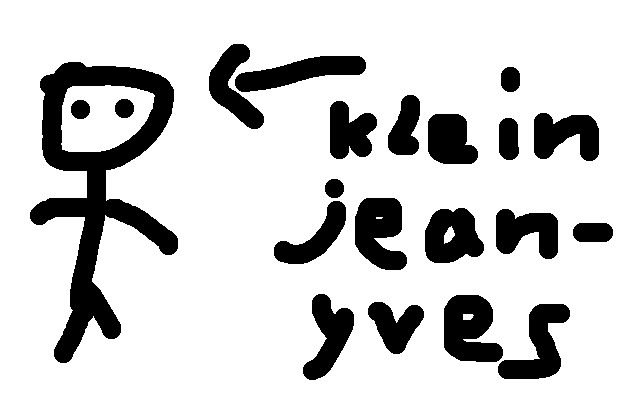
\includegraphics[width=\framewidth]{comic1.png}
\end{frame}
\begin{frame}
  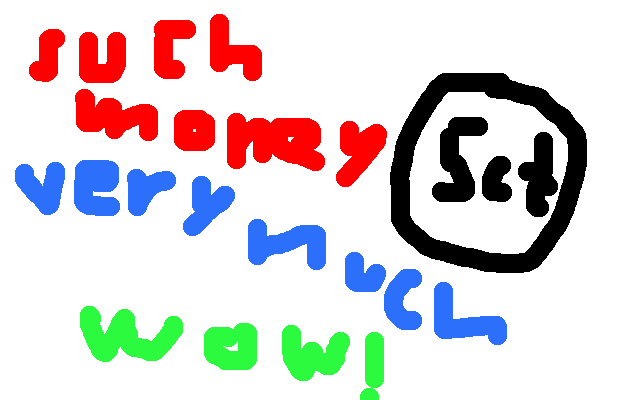
\includegraphics[width=\framewidth]{comic2.png}
\end{frame}
\begin{frame}
  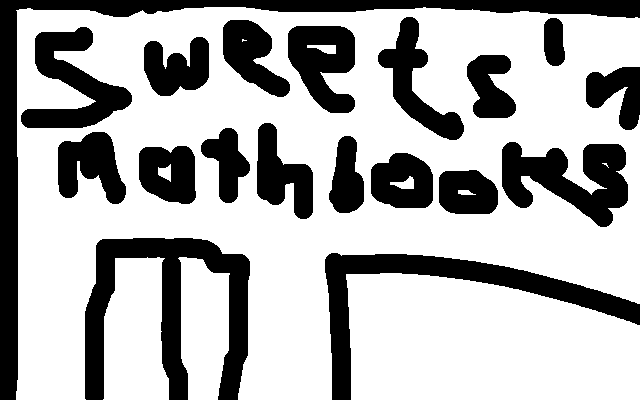
\includegraphics[width=\framewidth]{comic3.png}
\end{frame}
\begin{frame}
  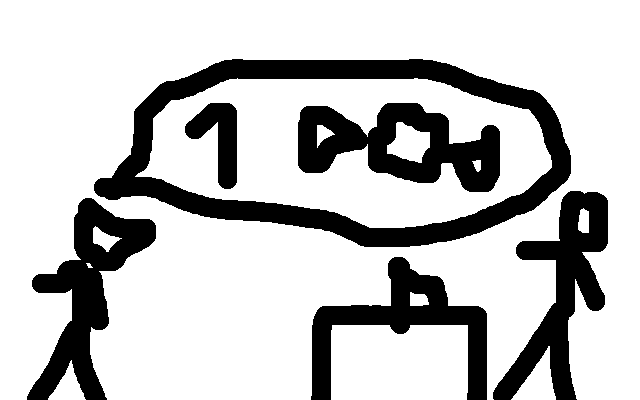
\includegraphics[width=\framewidth]{comic4.png}
\end{frame}
\begin{frame}
  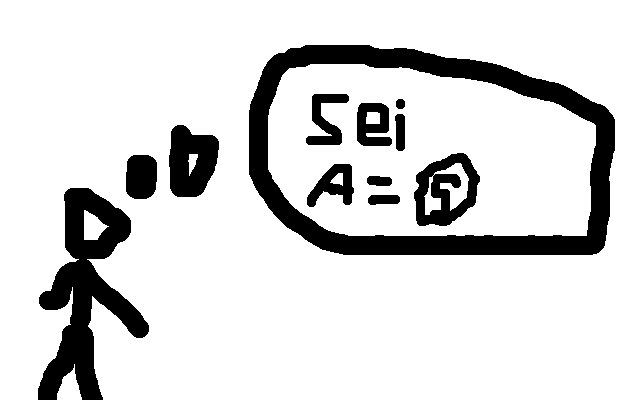
\includegraphics[width=\framewidth]{comic5.png}
\end{frame}
\begin{frame}
  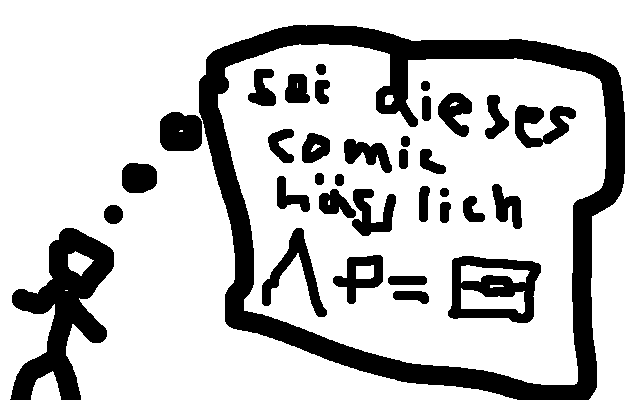
\includegraphics[width=\framewidth]{comic6.png}
\end{frame}
\begin{frame}
  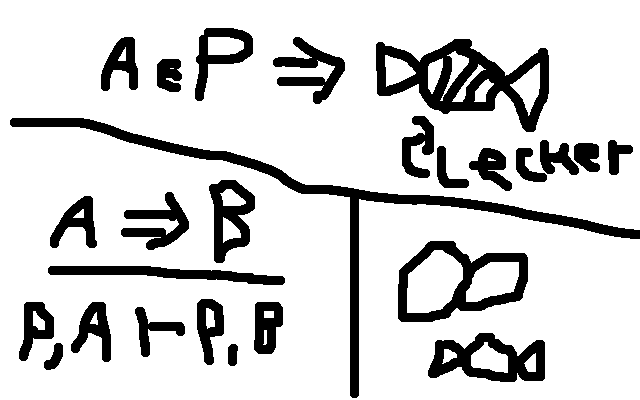
\includegraphics[width=\framewidth]{comic7.png}
\end{frame}

\begin{frame}
  \frametitle{Intuitionistisches Versagen}
  \textbf{Aussage A:} Jean-Yves hat 5 cent.\\
  \textbf{Aussage B:} Jean-Yves hat ein Bonbon.\\
  Ein Bonbon kostet 5 cent.\\ \pause%

  \begin{equation}
    \frac{A \implies B}
         {\Gamma, A \vdash \Gamma, B}
  \end{equation}
  
  \pause%
  
  \begin{equation}
    \frac{\Gamma \vdash B}
         {\Gamma, A \vdash B}
  \end{equation}
  
  \pause%
 
  \begin{equation}
    \frac{\Gamma, A, A \vdash B}
         {\Gamma, A \vdash B}
  \end{equation}

  \pause%

  \begin{equation}
    \frac{A \implies B}
         {\Gamma, A \vdash \Gamma, A, B}
  \end{equation}
\end{frame}

\begin{frame}
  \frametitle{Das Ziel von linearer Logik}
  \begin{itemize}[<+->]
    \item Resourcen sind endlich $\Rightarrow$ Jean-Yves bekommt nur ein Bonbon für 5 cent
    \item Wir müssen Resourcen sparen $\Rightarrow$ Jean-Yves darf nicht einfach Geld aus dem Fenster werfen
    \item Dennoch wollen wir alles ausdrücken können
  \end{itemize}
\end{frame}

\begin{frame}
  \frametitle{Eine kapitalistische Logik}

  Was, wenn wir auf diese Regeln verzichten?

  
  \begin{equation*}
    \frac{\Gamma \vdash B}
         {\Gamma, A \vdash B}
  \end{equation*}
 
  \begin{equation*}
    \frac{\Gamma, A, A \vdash B}
         {\Gamma, A \vdash B}
  \end{equation*}

\end{frame}

\begin{frame}
  \frametitle{Eine kapitalistische Logik}

  \begin{equation*}
    \frac{\Gamma, A, A \vdash B}
         {\Gamma, A \nvdash B}
  \end{equation*}

  Wir dürfen keine Resourcen verschwenden.

  \pause%

   \begin{equation*}
    \frac{\Gamma \vdash B}
         {\Gamma, A \nvdash B}
  \end{equation*}

  Wir dürfen keine Resourcen herbeizaubern, die für unseren „Kaufvorgang“ nicht relevant sind.
\end{frame}

\begin{frame}
  \frametitle{Lollis}
  Um keine Verwirrungen zwischen normalen Herleitungen zu verursachen, erfinden wir einen neuen Operator.
  
  \pause%

  Wir kennen bereits zwei Regeln die in der linearen Logik gelten:

  \pause%

  \begin{equation*}
    \frac{\Gamma \vdash B}
         {\Gamma, A \cancel{\multimap} B}
  \end{equation*}

  Jeder Wert \textbf{muss mindestens} ein mal verwendet werden.

  \pause%
  
  \begin{equation*}
    \frac{\Gamma, A, A \vdash B}
         {\Gamma, A \cancel{\multimap} B}
  \end{equation*}

  Jeder Wert \textbf{darf höchstens} ein mal verwendet werden.

\end{frame}

\begin{frame}
  \frametitle{Unendlichkeiten}
  Jean-Yves Großvater hat eine Solaranlage. Herr Girard fragt daher seinen Enkel Jean-Yves wie viel Strom die Anlage produziert.
  Jean-Yves ist die Antwort sofort klar. Sein Großvater hat unendlich viel Strom.

  \pause%

  Sei W = 1 Watt und Q = „Jean-Yves Großvater hat eine Solaranlage“. Intuitiv würde man sagen:

  \begin{equation}
    Q \multimap W
  \end{equation}

  \pause%

  Dann würde die Solaranlage allerdings verschwinden sobald sie 1 Watt produziert hat.
\end{frame}

\begin{frame}
  \frametitle{Of course!}
  Wir brauchen einen Weg, um zu sagen, dass eine Resource unendlich ist. \par
  $!A$ bedeutet, dass wir unendlich oft A haben. \par

  \pause%

  $!$ ist der „Of Course!“-Operator. \par
  
  \pause%

  Somit entsteht die Aussage:
  
  \begin{equation}
    Q \multimap !W
  \end{equation}
\end{frame}

\subsection{Lineare Operatoren}
\begin{frame}
  \frametitle{Tensor}
  \begin{equation}
    \frac{A \multimap B \qquad A \multimap C}
         {A, A \multimap B \otimes C}
  \end{equation}

  Jean-Yves kauft für 10ct Bonbons und Lollis.

  \pause%

  \begin{equation}
    \frac{A \vdash C \qquad B \vdash D}
         {A, B \vdash C \otimes D}
  \end{equation}

  \begin{equation}
    \frac{A \vdash B \otimes C \qquad \Gamma \vdash B, C \multimap D}
         {\Gamma, A \vdash D}
  \end{equation}
\end{frame}

\begin{frame}
  \frametitle{With}
  \begin{equation}
    \frac{A \multimap B \qquad A \multimap C}
         {A \multimap B \with C}
  \end{equation}

  Für 5ct bekommt Jean-Yves entweder Bonbons oder Lollis. Jean-Yves muss sich eines aussuchen.

  \pause%

  \begin{equation}
    \frac{A \vdash B \qquad A \vdash C}
         {A \vdash B \with C}
  \end{equation}

  \begin{equation}
    \frac{\Gamma \vdash A \with B}
         {\Gamma \vdash A}
  \end{equation}

  \begin{equation}
    \frac{\Gamma \vdash A \with B}
         {\Gamma \vdash B}
  \end{equation}
\end{frame}

\begin{frame}
  \frametitle{Plus}
  \begin{equation}
    \frac{A \multimap B}
         {A \multimap B \oplus C}
  \end{equation}

  Für 5ct kann Jean-Yves Bonbons oder Lollis kaufen. Leider sind die Lollis ausverkauft und Jean-Yves muss die Bonbons nehmen.

  \pause%

  \begin{equation}
    \frac{A \vdash B}
         {A \vdash B \oplus C}
  \end{equation}

  \begin{equation}
    \frac{A \vdash C}
         {A \vdash B \oplus C}
  \end{equation}

  \begin{equation}
    \frac{\Gamma \vdash A \oplus B \qquad \Delta \vdash A \multimap C \qquad \Delta \vdash B \multimap C}
         {\Gamma, \Delta \vdash C}
  \end{equation}
\end{frame}

\begin{frame}
  \frametitle{Par}
  Es gibt noch einen vierten Operator. Dieser lässt sich allerdings nicht so leicht erklären.

  \pause%

  \begin{equation*}
    A \parr B
  \end{equation*}

  A par B lässt sich in etwa so erklären, dass wir beide fälle behandeln müssen, A und B, allerdings wird nur eines von Beiden auftreten.

  \pause%

  Zum Beispiel kauft Jean-Yves Mutter Bonbons und Lollis, weil sie noch nicht weiß, welches von beidem Jean-Yves bevorzugt. Allerdings wird sie ihm nur eines von beidem geben.

  \begin{equation*}
    A \multimap B \parr C
  \end{equation*}
\end{frame}

\begin{frame}
  \frametitle{Spieltheorie}
  In der Spieltheorie haben die Operatoren eine interessante Bedeutung. \\~\\ \pause

  $A \oplus B$ bedeutet, dass wir an der Reihe sind und entweder A oder B spielen müssen. \\~\\ \pause
  $A \with B$ beudetet, dass der Gegner an der Reihe ist und entweder A oder P spielen muss. \\~\\ \pause

  $A \otimes B$ bedeutet, dass wir beide Spiele gleichzeitig spielen. Wenn wir in einem der Spiele am Zug sind, ist der Gegner in allen Spielen am Zug. Wenn wir in allen Spielen am Zug sind, dann sind wir am Zug. Nur, wenn wir beide Spiele gewinnen, haben wir gewonnen. Wenn eines der Spiele früher endet, geht das andere Spiel weiter.

  \\~\\ \pause
  $A \parr B$ ist dual dazu. Wir sind am Zug, außer der Gegner ist in beiden Spielen am Zug. Wenn wir in einem Spiel gewinnen, gewinnen wir alle Spiele. 
\end{frame}

\section{Lineare Typen}
\subsection{Curry-Howard Isomorphismus}
\begin{frame}
  \frametitle{Curry-Howard Isomorphismus}

  Der Curry Howard Isomorphismus sagt aus, dass sich logische Regeln in ein Typsystem wandeln lassen. Das funktioniert auch für lineare Logik.
\end{frame}

\begin{frame}
  \frametitle{Lineare Typen}
    
  \begin{equation}
    \frac{\Gamma \vdash x : A \multimap y : B}
         {\Gamma \vdash \lambda x.\ y : A \multimap B}
  \end{equation}

  \pause%

  \begin{equation}
    \frac{\Gamma \vdash f : A \multimap B \qquad \Delta \vdash x : A}
         {\Gamma, \Delta \vdash f(x) : B}
  \end{equation}
\end{frame}

\begin{frame}
  \frametitle{Tensor}
  \begin{equation}
    \frac{\Gamma \vdash x : A \qquad \Delta \vdash y : B}
         {\Gamma, \Delta \vdash (x, y) : A \otimes B}
  \end{equation}

  \pause%

  \begin{equation}
    \frac{\Gamma \vdash t : A \otimes B \qquad \Delta \vdash x : A,\ y : B \multimap s : C}
         {\Gamma, \Delta \vdash case\ t\ of\ (x, y) \rightarrow s : C}
  \end{equation}
\end{frame}

\begin{frame}
  \frametitle{With}
  \begin{equation}
    \frac{\Gamma \vdash x : A \qquad \Gamma \vdash y : B}
         {\Gamma \vdash [x,y] : A \with B}
  \end{equation}

  \pause%

  \begin{equation}
    \frac{\Gamma \vdash t : A \with B}
         {\Gamma \vdash fst(t) : A}
  \end{equation}

  \begin{equation}
    \frac{\Gamma \vdash t : A \with B}
         {\Gamma \vdash snd(t) : B}
  \end{equation}
\end{frame}

\begin{frame}
  \frametitle{Plus}
  \begin{equation}
    \frac{\Gamma \vdash x : A}
         {\Gamma \vdash Left\ x : A \oplus B}
  \end{equation}
  \begin{equation}
    \frac{\Gamma \vdash x : B}
         {\Gamma \vdash Right\ x : A \oplus B}
  \end{equation}

  \pause%

  \begin{equation}
    \frac{\Gamma \vdash c : A \oplus B \qquad \Delta \vdash x : A \multimap t : C \qquad \Delta \vdash y : B \multimap u : C}
         {\Gamma, \Delta \vdash case\ c\ of\ Left\ x \rightarrow t; Right\ y \rightarrow u : C}
  \end{equation}
\end{frame}

\subsection{Haskell}
\begin{frame}[fragile]
  \frametitle{Lineare Typen in Haskell}
  In Haskell gibt es ein Proposal zu linearen Typen. Dabei schreibt man in den Typen noch wie häufig ein Wert benutzt werden darf.

  \begin{lstlisting}
    data Tensor a b =
      Tensor { tensorFirst ::1 a
             , tensorSecond ::1 b
             }
  \end{lstlisting}

  \begin{lstlisting}
    linearMap :: (a -o b) -> f a -o f b
  \end{lstlisting}
\end{frame}

\begin{frame}
  \begin{equation*}
    Vortrag \multimap Ende
  \end{equation*}
\end{frame}

\end{document}
